\section{Experiments}
\subsection{Data Source}
We perform the researcher future citation prediction on the Google Scholar database.
It covers *** publications by *** researchers for more than 50 years.
The total number of citations is roughly *** in this data set.

We used all papers with cross validation to formulate the publication level future citation prediction model.
With this model we created a new feature that aggregates all the number of citation predicted from all papers a researcher published before year $t$.

For each researcher who has been active for at least $\Delta t$ years, we generate a new record in a new data set for each year after the first $\Delta t$ years, i.e. if a researcher has been active for 40 years and $\Delta t=5$. 35 records are generated for every year after five years in the field. 

Since our work is time independent, therefore, we randomly split the data with 50\% for training, 20\% validation and another 30\% for test. 

We compare our predicted future citations with actual future citations in the test set.

\subsection{Evaluation}
The coefficient of determination ($R^2$) is used in evaluating how well prediction model fits the test data.
The definition of $R^2$ is:
\[R^2=\frac{\sum_{r \in }\hat{D_c}(r,t,\Delta t)-\bar{D_c}}{}\]
where $\hat{D_c}$ is the predicted future citation for researcher $r$ in year $t$, 
and $\bar{D_c}$ represents the mean of the actual citations from year $t$ to $t+\Delta t$ for all researchers.

By definition, $R^2\in [0,1]$, with $R^2=0$ means the predicted citations does not fit the actual citations at all,
and $R^2=1$ means the model perfectly predicted the future citations. A model with a larger $R^2$ indicates a better prediction performance and is therefore desired. 
\subsection{Prediction Performance}
Following Yan et al.'s work, our prediction model for publication future citation is summarized in table \ref{tbl-pubprediction}.

\begin{table}[!h]
\begin{center}
\begin{tabular}{c|c|c|c|c|c}
\hline
$R^2$& LR & DFR & PR & LASSO & Ridge\\
\hline
$\Delta t=1$ & & & & &\\
\hline
$\Delta t=5$ & & & & &\\
\hline
$\Delta t=10$ & & & & &\\
\hline
\end{tabular}
\end{center}
\caption{Publication future citation prediction evaluation}
\label{tbl-pubprediction}

\end{table}

The prediction for researcher future citations is summarized in table \ref{tbl-r2}.
The best predictive performance for next five year researcher citations is plotted in figure \ref{researcher-prediction}.


\begin{figure}
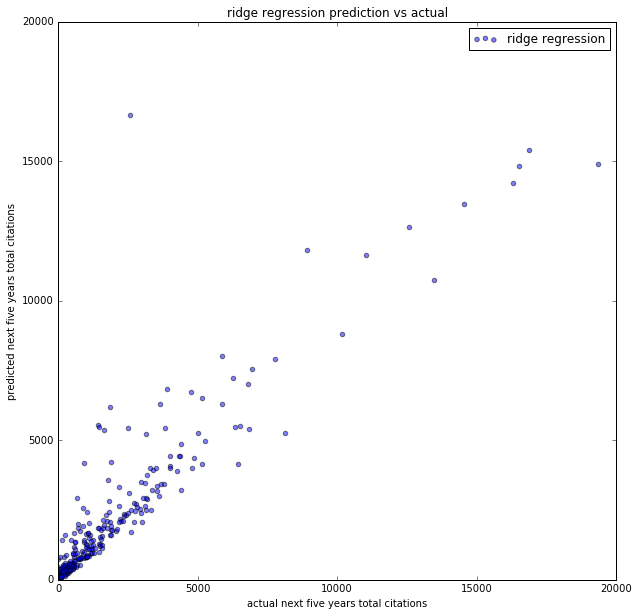
\includegraphics[width=3 in]{fig/researcher-prediction.png}
\caption{Ridge Regression on researcher next five years prediction.}
\label{researcher-prediction}
\end{figure}

\begin{table*}[t]
\begin{center}
\begin{tabular}{c|c|c|c|c|c|c|c|c|c|c|c|c|c|c|c}
\hline
& \multicolumn{5}{|c|}{\textbf{$\Delta t =1$}}& \multicolumn{5}{|c|}{$\Delta t =5$}& \multicolumn{5}{|c}{$\Delta t =10$}\\

\hline
Methods & LR & DFR & PR & SVR & R& LR & DFR & PR & SVR & R& LR & DFR & PR & SVR & R\\
\hline\hline
+org.Rank & & & & & & & & & & & & & & & \\
\hline
+$N_c(r,t)$ & & & & & & & & & & & & & & & \\
\hline
+index & & & & & & & & & & & & & & & \\
\hline
+years & & & & & & & & & & & & & & & \\
\hline\hline
-org.Rank & & & & & & & & & & & & & & & \\
\hline
-$N_c(r,t)$ & & & & & & & & & & & & & & & \\
\hline
-index & & & & & & & & & & & & & & & \\
\hline
-years & & & & & & & & & & & & & & & \\
\hline\hline
Combined & & & & & & & & & & & & & & & \\
\hline
\end{tabular}
\end{center}
\caption{The performance of various predictive models on the test set."+""-"}
\label{tbl-r2}

\end{table*}



\subsubsection{Variance in Prediction}
As we can see, most of the variance in our predictive model are having a higher predicted future citations than actual. This may result from unpredictable situations, for example, the retirement of a researcher. 

Sidiropoulos et al. reported that h-index has shortcomings in what majorly of its inability to distinguish active and inactive(retired) researchers\cite{sidiropoulos2007generalized}. The higher h-index contributes as a positive factor in our prediction and results in a higher prediction. In our work this also reflects the potential lack of knowledge of the recent status of researchers.
{\sc still need explanation.}

\subsubsection{Citation Distribution}
As is shown in figure \ref{researcher-prediction}, the distribution of future researchers citations shows a long tail. 
Most researchers gets a total future citations less than 2,500 cites.

\subsubsection{Factor Contribution}
{\it Most Useful Feature}

{\it publication level prediction}

































